%% Submissions for peer-review must enable line-numbering 
%% using the lineno option in the \documentclass command.
%%
%% Preprints and camera-ready submissions do not need 
%% line numbers, and should have this option removed.
%%
%% Please note that the line numbering option requires
%% version 1.1 or newer of the wlpeerj.cls file.

\documentclass[fleqn,10pt,lineno]{wlpeerj} % for journal submissions
% \documentclass[fleqn,10pt]{wlpeerj} % for preprint submissions

\title{An Empirical Study on Combining Active Learning Suggestions}

\author[1]{Alasdair Tran}
\author[2]{Cheng Soon Ong}
\affil[1]{Data to Decisions CRC, Kent Town, SA 5067, Australia}
\affil[2]{Machine Learning Research Group, Data61, CSIRO, Australia}

\keywords{machine learning, astronomy, active learning, bandit, rank aggregation}

\begin{abstract}
Recent advances in sensors and scientific instruments have led to an increasing use of machine learning techniques for managing the data deluge. Supervised learning has become a widely used paradigm in many big data applications. However,  labeled examples are required during the training phase of supervised machine learning algorithms, and the labeling has become a significant bottleneck. This paper explores the use of machine learning algorithms for identifying informative examples for labeling, the so-called active learning setting. We empirically compare several active learning heuristics on benchmark datasets, and focus on its application to photometric classification of the Sloan Digital Sky Survey. By considering each active learning heuristic as an expert recommendation of which example to label, we propose to combine them using bandit and rank aggregation algorithms. Our results show that combining active learning suggestions improves over each individual heuristic (including passive learning), and provides a promising practical approach.
\end{abstract}

\begin{document}

\flushbottom
\maketitle
\thispagestyle{empty}

\section*{Introduction}

Your introduction goes here! Some examples of commonly used commands and features are listed below, to help you get started.

If you have a question, please use the help menu in the top right of the screen to get in touch. When your article or pre-print is complete, use the "Submit to PeerJ" button in the topbar to send your files to PeerJ.

\subsection*{About PeerJ}

PeerJ is an award-winning open access publisher covering the biological and medical sciences.  PeerJ provides authors with three publication venues: \textit{PeerJ} and \textit{PeerJ Computer Science} (peer-reviewed academic journals) and \textit{PeerJ PrePrints} (a 'pre-print server'). See https://peerj.com/about/publications/ for more information.

The PeerJ model allows an author to publish articles in their peer-reviewed journal via the purchase of a lifetime Publication Plan. Prices start from just \$99 (a one-off payment) which entitles an author to the lifetime ability to publish 1 article per year for free. Publication in PeerJ PrePrints is entirely free.

\section*{Some \LaTeX{} Examples}
\label{sec:examples}

Use section and subsection commands to organize your document. \LaTeX{} handles all the formatting and numbering automatically. Use ref and label commands for cross-references.

\subsection*{Figures and Tables}

Use the table and tabular commands for basic tables --- see Table~\ref{tab:widgets}, for example. You can upload a figure (JPEG, PNG or PDF) using the project menu. To include it in your document, use the includegraphics command as in the code for Figure~\ref{fig:view} below.

\begin{figure}[ht]
\centering
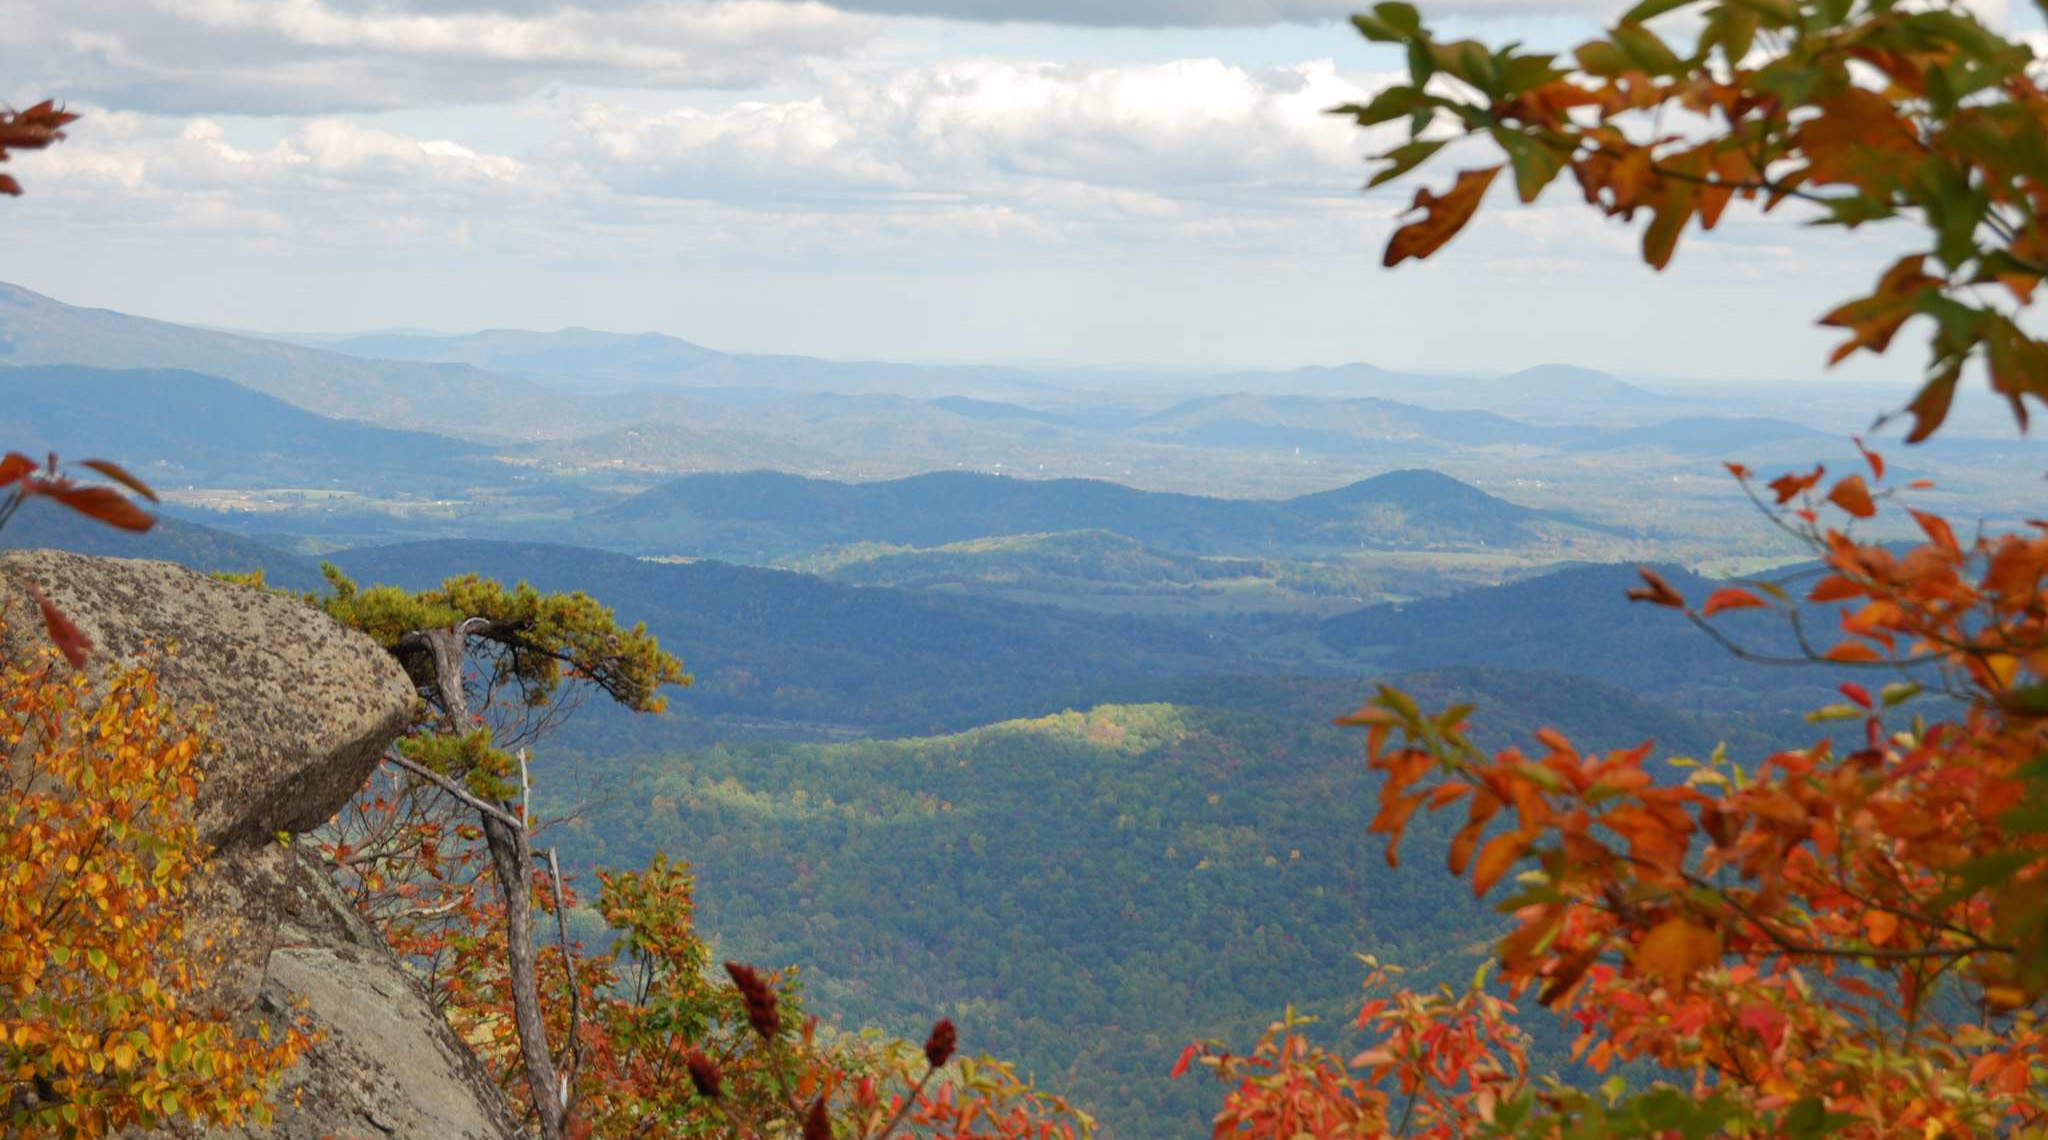
\includegraphics[width=\linewidth]{view}
\caption{An example image.}
\label{fig:view}
\end{figure}

\begin{table}[ht]
\centering
\begin{tabular}{l|r}
Item & Quantity \\\hline
Widgets & 42 \\
Gadgets & 13
\end{tabular}
\caption{\label{tab:widgets}An example table.}
\end{table}

\subsection*{Citations}

LaTeX formats citations and references automatically using the bibliography records in your .bib file, which you can edit via the project menu. Use the cite command for an inline citation, like \cite{Figueredo:2009dg}, and the citep command for a citation in parentheses \citep{Figueredo:2009dg}.

\subsection*{Mathematics}

\LaTeX{} is great at typesetting mathematics. Let $X_1, X_2, \ldots, X_n$ be a sequence of independent and identically distributed random variables with $\text{E}[X_i] = \mu$ and $\text{Var}[X_i] = \sigma^2 < \infty$, and let
$$S_n = \frac{X_1 + X_2 + \cdots + X_n}{n}
      = \frac{1}{n}\sum_{i}^{n} X_i$$
denote their mean. Then as $n$ approaches infinity, the random variables $\sqrt{n}(S_n - \mu)$ converge in distribution to a normal $\mathcal{N}(0, \sigma^2)$.

\subsection*{Lists}

You can make lists with automatic numbering \dots

\begin{enumerate}[noitemsep] 
\item Like this,
\item and like this.
\end{enumerate}
\dots or bullet points \dots
\begin{itemize}[noitemsep] 
\item Like this,
\item and like this.
\end{itemize}
\dots or with words and descriptions \dots
\begin{description}
\item[Word] Definition
\item[Concept] Explanation
\item[Idea] Text
\end{description}

We hope you find write\LaTeX\ useful for your PeerJ submission, and please let us know if you have any feedback. Further examples with dummy text are included in the following pages.

\section*{Methods}

\lipsum[4] % Dummy text

\begin{equation}
\cos^3 \theta =\frac{1}{4}\cos\theta+\frac{3}{4}\cos 3\theta
\label{eq:refname2}
\end{equation}

\lipsum[5] % Dummy text

\subsection*{Subsection}

\lipsum[6] % Dummy text

\paragraph{Paragraph} \lipsum[7] % Dummy text
\paragraph{Paragraph} \lipsum[8] % Dummy text

\subsection*{Subsection}

\lipsum[9] % Dummy text

\begin{figure}[ht]\centering
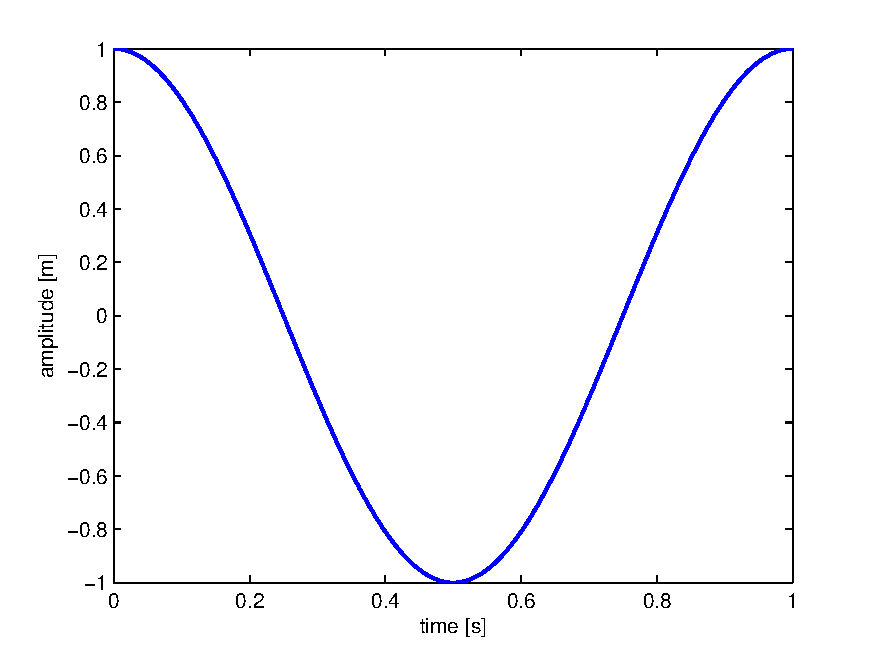
\includegraphics[width=\linewidth]{results}
\caption{In-text Picture}
\label{fig:results}
\end{figure}

Reference to Figure \ref{fig:results}.

\section*{Results and Discussion}

\lipsum[10] % Dummy text

\subsection*{Subsection}

\lipsum[11] % Dummy text

\subsubsection*{Subsubsection}

\lipsum[12] % Dummy text

\subsubsection*{Subsubsection}

\lipsum[14] % Dummy text

\subsection*{Subsection}

\lipsum[15-20] % Dummy text

\section*{Acknowledgments}

So long and thanks for all the fish.

\bibliography{sample}

\end{document}